% !Rnw root = learnR.Rnw




A first step is to load the \textit{tm} package.  This is designed for
working with collections of documents, where a collection has the name
\texttt{Corpus}.
\begin{Schunk}
\begin{Sinput}
library(tm)
\end{Sinput}
\end{Schunk}

\section{Creation of a Volatile Corpus}\label{sec:volatile}

\marginnote[11pt]{A pdf to text converter has taken the pdf for this
  document, and extracted the three chapter ranges into the
  respective files {\bf ch1-5prelims.txt}, {\bf ch6-7data.txt}, and
  {\bf ch8-9graphics.txt}.}

The data used is from three text files, stored in the {\em DAAGviz}
directory tree.  They hold text from the respective chapter ranges 1 -
5, 6 - 7, and 8 - 9 of this present document.  We show two ways to use
it to form a corpus.  The first breaks the process down into detailed
steps, while the second uses a much terser and summary approach.  The
resultant corpus is {\em volatile}, so described because stored in the
workspace.  Unless saved separately or as part of the workspace, it
will disappear at the end of the session.

\subsection*{Detailed steps}

First create paths to the files, and check that they seem correct:
\begin{fullwidth}
\begin{Schunk}
\begin{Sinput}
## Create paths to the files
txdir <- system.file("texts", package="DAAGviz")
dir(txdir, pattern=".txt$")
\end{Sinput}
\begin{Soutput}
[1] "data6-7.txt"     "graphics8-9.txt" "prelims1-5.txt" 
\end{Soutput}
\begin{Sinput}
txfiles <- dir(txdir, pattern=".txt$", full.names=TRUE)
\end{Sinput}
\end{Schunk}
\begin{Schunk}
\begin{Sinput}
## Input first file, with one text string per line
tx1 <- readLines(txfiles[1], encoding="UTF-8", warn=FALSE)
## Join the separate text strings end to end
tx1 <- paste(tx1, collapse=" ")
\end{Sinput}
\end{Schunk}
\end{fullwidth}

Repeat this process for files 2 and 3:
\begin{fullwidth}
\begin{Schunk}
\begin{Sinput}
tx2 <- readLines(txfiles[2], encoding="UTF-8", warn=FALSE)
tx2 <- paste(tx2, collapse=" ")
tx3 <- readLines(txfiles[3], encoding="UTF-8", warn=FALSE)
tx3 <- paste(tx3, collapse=" ")
\end{Sinput}
\end{Schunk}
\end{fullwidth}

Now bring the three text strings together into a corpus:
\begin{Schunk}
\begin{Sinput}
txcorp <- Corpus(VectorSource(c(tx1, tx2, tx3)))
\end{Sinput}
\end{Schunk}

\subsection*{Creation of a corpus using \txtt{DirSource()}}

\marginnote{The call to \margtt{tm\_map()} is a mechanism for marking the
  document as UTF-8. The pdf to text converter creates UTF-8
  documents.  The tokenizer \margtt{scan\_takenizer} then calls
  \margtt{scan()}, but without marking the document that results as
  UTF-8, as required for use of \margtt{termDocumentMatrix()} or
  \txtt{termFreq()}.}
The following creates a directory source:
\begin{Schunk}
\begin{Sinput}
dirSource <- DirSource(directory=txdir,
                       pattern=".txt$")
\end{Sinput}
\end{Schunk}

Now create the corpus.  The text will be input from the files that
were identified, within the specified directory {\bf doc}:
\begin{Schunk}
\begin{Sinput}
toUTF8 <- function(x) iconv(x, to="UTF-8",
                            sub = "byte")
txcorp <- Corpus(dirSource)
txcorp <- tm_map(txcorp,
    content_transformer(toUTF8))
\end{Sinput}
\end{Schunk}

\subsection*{Next steps}

A common starting point for further work is a term by document matrix.
For this, use \txtt{TermDocumentMatrix()}.  Or if a
document by term matrix is required, use \txtt{DocumentTermMatrix()}

%' \begin{marginfigure}[12pt]
%'   Alternatively, make repeated use of \margtt{tm\_map()} to
%'   operate directly on the corpus, thus:
%' <<tm-map, eval=FALSE>>=
%' @ %
%' \end{marginfigure}
Pre-processing steps prior to creating such a matrix may include
stripping away stopwords, elimination of white space, and conversion
to lower case.  These can be performed in the process of creating a
term document matrix, thus:
\begin{fullwidth}
\begin{Schunk}
\begin{Sinput}
ctl <- list(stopwords = c(stopwords(), "[1]"),
            removePunctuation = list(preserve_intra_word_dashes = FALSE),
            removeNumbers = TRUE, stopwords=c(stopwords(), "[1]"),
            minDocFreq = 2)
tx.tdm <- TermDocumentMatrix(txcorp, control=ctl)
\end{Sinput}
\end{Schunk}
\end{fullwidth}
\noindent
Notice the identification of \txtt{[1]}, which appears quite
frequently in the R output, as a stopword.  This omits it from the
list of terms.  Closer investigation would reveal other issues, most
because the default tokenizer\sidenote{See \margtt{help(termFreq)} for
  an example of a user-supplied tokenizer.} is not designed to handle
R code and output.

Now list terms that occur 100 or more times:
\begin{fullwidth}
\begin{Schunk}
\begin{Sinput}
findFreqTerms(tx.tdm, 100)
\end{Sinput}
\begin{Soutput}
 [1] "can"       "code"      "data"      "figure"    "file"     
 [6] "frame"     "function"  "functions" "graphics"  "objects"  
[11] "package"   "plot"      "use"       "used"      "using"    
[16] "will"     
\end{Soutput}
\end{Schunk}
\end{fullwidth}

\subsection*{Wordclouds}

First load the {\em wordcloud} package:
\begin{Schunk}
\begin{Sinput}
library(wordcloud)
\end{Sinput}
\end{Schunk}

Figure \ref{fig:wc} shows wordcloud plots for the first (chapters 1-5),
second (6-7) and third (8-9) documents in the corpus.
\vspace*{15pt}

\begin{figure*}
\begin{Schunk}


\centerline{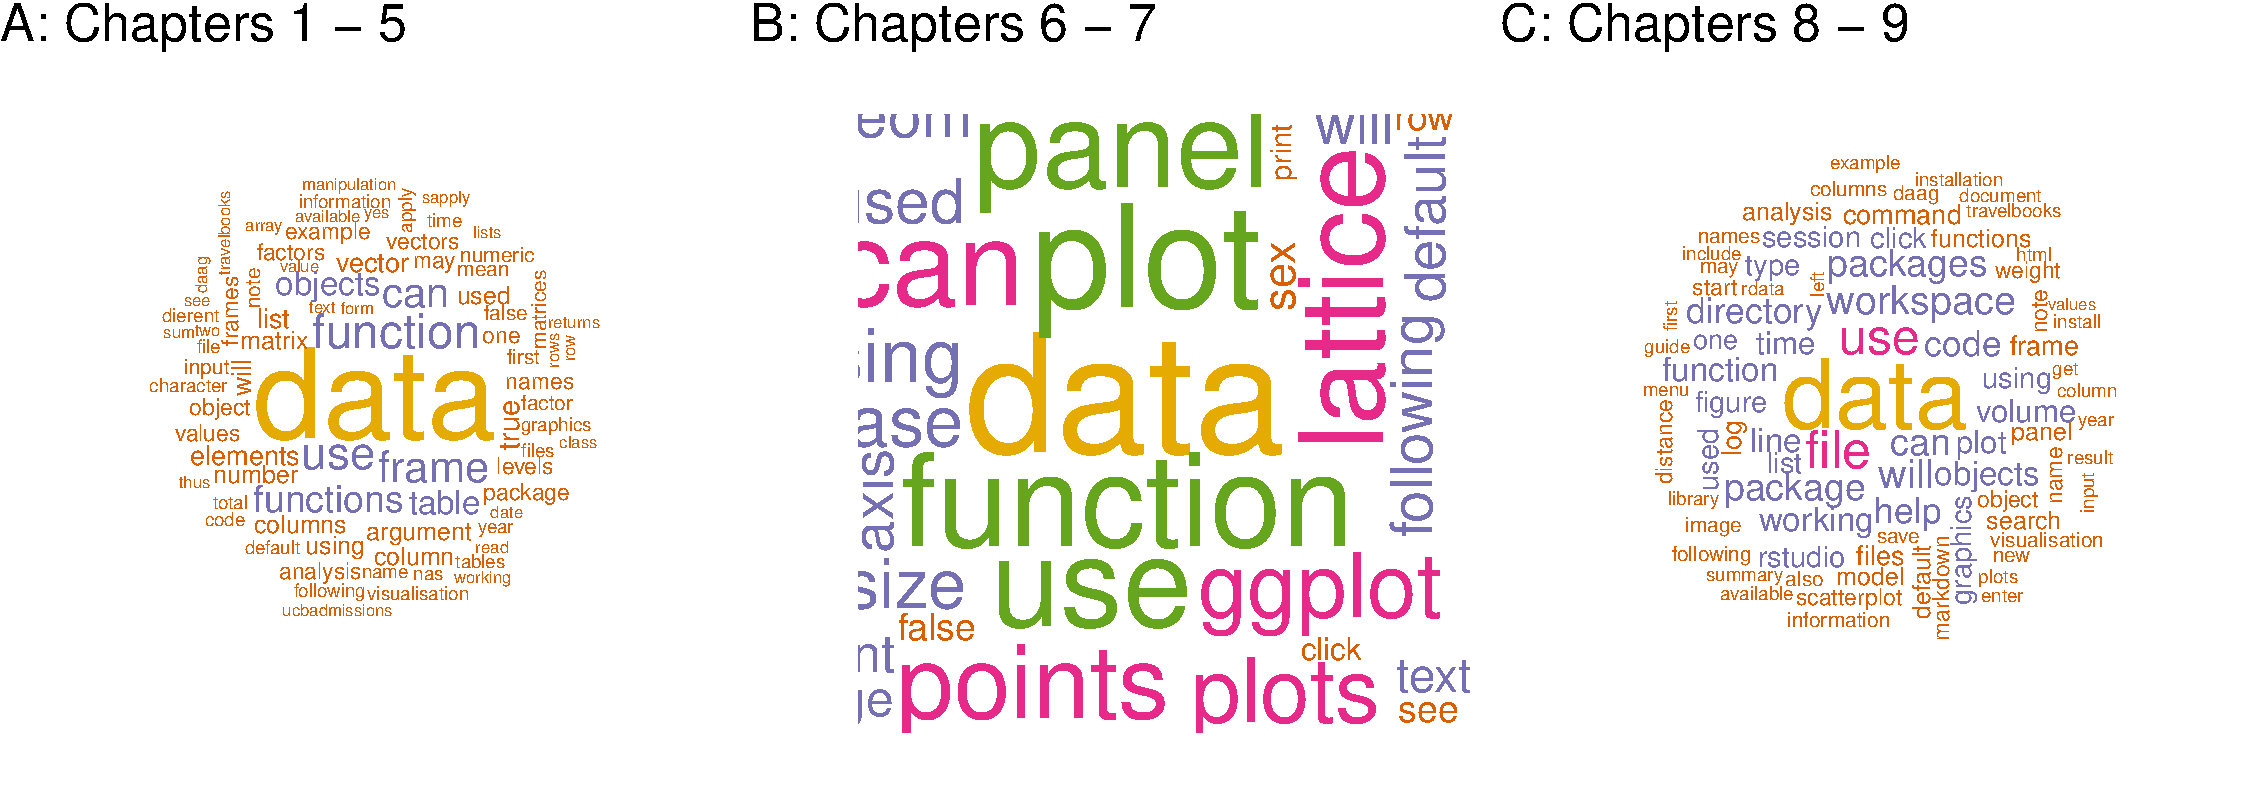
\includegraphics[width=0.92\textwidth]{figs/14-wordcloud1-3-1} }

\end{Schunk}
\caption[][-12pt]{Wordcloud plots are A: for the words in Chapters 1 - 5; B: 6 -
  7; and C: 8 - 9. For a color version of Panel A, see Figure 
  \ref{fig:cloudfun}.\label{fig:wc}}
\setfloatalignment{b}
\end{figure*}

\vspace*{-9pt}

\noindent
Code for the plots is:
\begin{fullwidth}
\begin{Schunk}
\begin{Sinput}
pal <- brewer.pal(6, "Dark2")
fnam1 <- as.matrix(tx.tdm)[,1]
wordcloud(names(fnam1), fnam1, max.words=80, colors=pal[-1],
          random.order=FALSE, scale=c(6.5,.5))
mtext(side=3, line=3.5, "A: Chapters 1 - 5", adj=0, cex=1.8)
fnam2 <- as.matrix(tx.tdm)[,2]
wordcloud(names(fnam2), fnam2, max.words=80, colors=pal[-1],
          random.order=FALSE, scale=c(10,.5))
mtext(side=3, line=3.5, "B: Chapters 6 - 7", adj=0, cex=1.8)
fnam3 <- as.matrix(tx.tdm)[,3]
wordcloud(names(fnam3), fnam3, max.words=80, colors=pal[-1],
          random.order=FALSE, scale=c(5,.5))
mtext(side=3, line=3.5, "C: Chapters 8 - 9", adj=0, cex=1.8)
\end{Sinput}
\end{Schunk}
\end{fullwidth}
\marginnote[12pt]{All three panels used a 5in by 5in graphics page,
  with a pdf pointsize of 12.} Less frequent words will be lost off the
edge of the plot if the size of the graphics page is too small
relative to the pointsize.  Note the different scaling ranges used in
the three cases, with the large scaling range for Panel B
(\txtt{scale=c(10,.5)}) used to accommmodate a frequency distribution
in which one item (`data') is a marked outlier.

\section{Creation of a Corpus from PDF Files}

The {\em tm} package has functions that can be used to create readers
for several different types of files.  Type \txtt{getReaders()} to get
a list.  Note in particular \txtt{readPDF()} that can be used with pdf
files.  For use of this command, both the tools pdfinfo and pdftotext
must be installed and accessible.  These are available as command line
utilities in the Poppler PDF rendering library (see
\url{http://poppler.freedesktop.org/}).

The following reads in the text from the file {\bf ch1-5prelims.pdf}.
The result is equivalent to using \txtt{readLines()} as above to
input lines from the text file {\bf ch1-5prelims.txt}:
\begin{Schunk}
\begin{Sinput}
uri <- "doc/ch1-5prelims.pdf"
pdfReadFun <- readPDF(PdftotextOptions = "-layout")
txx1 <- pdfReadFun(elem = list(uri = uri),
                   language = "en", id = "prelims")
\end{Sinput}
\end{Schunk}

The corpus that has all three documents is, starting with the
pdf files, most easily created thus:
\begin{fullwidth}
\begin{Schunk}
\begin{Sinput}
txXpdf <- Corpus(DirSource(directory="doc", pattern=".pdf$"),
                 readerControl=list(reader=readPDF,
                 PdftotextOptions = "-layout"))
\end{Sinput}
\end{Schunk}
\end{fullwidth}

\section{Document Collections Supplied With {\em tm}}
Several document collections are supplied with the package,
as text files or as XML files.  To get the path to the
directories where these document collections are stored, type
\begin{fullwidth}

\begin{Schunk}
\begin{Sinput}
(pathto <- system.file("texts", package="tm"))
\end{Sinput}
\begin{Soutput}
[1] "/Users/johnm1/Library/R/3.4/library/tm/texts"
\end{Soutput}
\begin{Sinput}
dir(pathto)
\end{Sinput}
\begin{Soutput}
[1] "acq"               "crude"             "custom.xml"       
[4] "loremipsum.txt"    "rcv1_2330.xml"     "reuters-21578.xml"
[7] "txt"              
\end{Soutput}
\end{Schunk}

\end{fullwidth}
The subdirectory \textbf{acq} has 50 Reuters documents in XML format,
\textbf{crude} has the first 23 of these, and \textbf{txt} has a
small collection of 5 text documents from the Roman poet Ovid.
These can be accessed and used for experimenation with the abilities
provided in {\em tm}, as required.

The following are the names of the five Ovid documents:
\begin{fullwidth}

\begin{Schunk}
\begin{Sinput}
dir(paste(pathto, "txt",sep="/"))
\end{Sinput}
\begin{Soutput}
[1] "ovid_1.txt" "ovid_2.txt" "ovid_3.txt" "ovid_4.txt" "ovid_5.txt"
\end{Soutput}
\end{Schunk}

\end{fullwidth}

The following brings these documents into a volatile corpus, i.e.,
a corpus that is stored in memory:
\begin{Schunk}
\begin{Sinput}
(ovid <-
   Corpus(DirSource(paste(pathto, "txt", sep="/")),
          readerControl=list(language="lat")))
\end{Sinput}
\begin{Soutput}
<<SimpleCorpus>>
Metadata:  corpus specific: 1, document level (indexed): 0
Content:  documents: 5
\end{Soutput}
\end{Schunk}

